\chapter{Experimentos numéricos}
\label{ch:chapter4}
 
En este capítulo se muestran los resultados obtenidos de la implementación del algoritmo de Newton-Lanczos, el cual se usó para maximizar el cociente planteado por el ADLF (Análisis Discriminante Lineal de Fisher). Este método encuentra la matriz de proyección óptima que maximiza el cociente de la matriz de dispersión entre clases y la matriz de dispersión intra clase. Maximizar esta formulación  tiene como resultado que la proyección mantenga a los individuos de una misma clase cercanos uno a otro además que mantiene alejados a los centroides de las distintas clases. 

Como se mencionó en capítulos anteriores, el ADLF es un método de reducción dimensional previo a un algoritmo de clasificación. Esta reducción dimensional es importante en problemas de dimensionalidad alta, ya que pueden reducir el problema a uno mucho más sencillo y computacionalmente eficiente. El aumento en la eficiencia computacional se debe a que se trabaja sobre un espacio de menor dimensionalidad, por lo que las operaciones a realizar son más rápidas. Otros problemas como \textit{The curse of dimensionality} también se ven solucionados. Esto tiene consecuencias computaciones inmediatas, en particular para métodos que requieren el cómputo exhaustivo de distancias como \textit{k-vecinos más cercanos}. Por esto motivo, en esta tesis, se utiliza esta técnica para calcular la probabilidad de pertenencia a cada clase.

Para comparar la precisión y el tiempo de cómputo del método de ADLF implementado con el algoritmo de Newton-Lanczos en problemas de dimensionalidad alta se comparará con otros dos métodos que realizan clasificación lineal: el Análisis Discriminante Lineal (ADL) y la Regresión Logística Multinomial (RLM). Estos métodos se seleccionaron debido a que tienen un fuerte fundamento teórico y han sido probados en múltiples conjuntos de datos. Para comparar estos métodos se utilizaron dos conjuntos de datos, los cuales fueron cuidadosamente seleccionados para ejemplificar las ventajas del ADLF. Una de las características buscadas en estos conjuntos de datos fue que presentaran dimensionalidad alta; es decir, un alto número de variables. La otra característica que se consideró para seleccionar la base de datos fue que clasificación lineal sea adecuada al problema.

La primer base de datos utilizada fue liberada por la compañia aseguradora \textit{State Farm}, la cual consiste en fotografías de conductores distraídos mientras manejan. El objetivo de la compañía al liberar esta base de datos fue contar con un clasificador de individuos que permitiera asignarlo a distintos grupos de riesgo de acuerdo a sus hábitos de manejo. Para lograr esto, se debe clasificar correctamente cada imagen de acuerdo a la actividad que está realizando (hablar por telefono, cambiar estación de radio, mandar mensajes de texto, etc.). En esta imagen las variables tomadas en cuenta fueron los píxeles; es decir, cada píxel se convirtió en una variable.

La segunda base de datos utilizada fue liberada por una de las compañías más grandes de comercio electrónico del mundo: \textit{Otto group}. Esta empresa actualmente tiene problemas para clasificar sus productos en 9 grupos dependiendo de 93 variables de las cuales no reveló la información de cada una. Como consecuencia no se puede realizar \textit{feature extraction} ya que se desconoce la información brindada por cada variable. 

El capítulo se divide en cinco partes. En la sección 3.1 se compara el tiempo de cómputo del método de Lanczos con reortogonalización completa para calcular los eigenpares de una matriz con el tiempo de la rutina $SVD$ de R. \footnote{La rutina $svd$ de $R$ ocupa la función $gesdd$ de la librería $LAPACK$. Para más información puede consultarse la página $http://www.netlib.org/lapack/$.}. En la sección 3.2, se explica el preprocesamiento de las bases de datos y el proceso para crear los conjuntos de entrenamiento y prueba. En la sección 3.3 y 3.4 se realizan los experimentos con la bases de \textit{State Farm} y \textit{Otto group} respectivamente. Al final, se presentan las conclusiones de los experimentos numéricos.

Para calcular los resultados presentados en este capítulo se utilizó el lenguaje de programación \textsf{R} en su versión 3.3.0 \textit{Supposedly Educational}. Los cálculos fueron realizados en una iMac 3.2 Ghz Intel Core i3 con 12 GB de RAM.

\section{Comparación de tiempo entre el método de Lanczos y la factorización SVD}

Como se mostró en el capítulo anterior, la parte central del algoritmo de Newton-Lanczos involucra la maximización del cociente de trazas. Para lograrlo es necesario calcular los primeros eigenpares de una resta de matrices. Estos pueden ser calculados con el método de Lanczos o con la factorización $SVD$, por lo que acontinuación se mostrará una breve comparación de ambos métodos. Es importante recordar que el método de Lanczos en aritmética exacta realiza eficientemente estos cálculos, pero en aritmética inexacta requiere la reortogonalización de los eigenvectores calculados, proceso que toma tiempo. 

Para ejemplificar las ventajas comparativas de los métodos se realizará un experimento numérico. La matriz utilizada para la prueba es $A - \rho B$ con $A$ y $B$ la matriz de dispersión intra clase y la matriz de dispersión entre clases de la base de datos de \textit{State Farm} respectivamente. $\rho$ se tomo en particular con el valor de 3. Ambas matrices tienen una dimensionalidad de $400 \times 400$. La siguiente gráfica resume el desempeño de ambos métodos cuando se desean calcular los primeros $1, 2, 3, 4, 5, 6, 7, 8, 9, 10, 20, 30, 40, 50, 70, 80,  90, 100,  110, 120$ componentes principales de la matriz en cuestión.

\pagebreak

\begin{figure}[!ht]
  \centering
  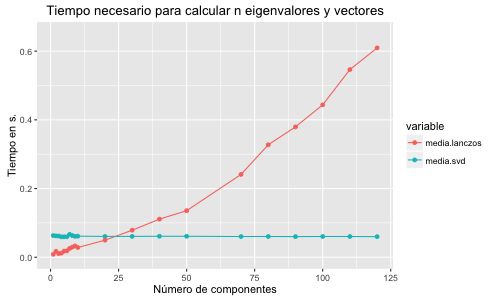
\includegraphics[width=1\textwidth]{Figures/Chapter4_eigen_lanczos_actuaria.png} 
  \caption[Desempeño de Lanczos]
  {En el eje $x$ se representa $k$, el número de eigenpares a calcular de la matriz $A- \rho B$. La matriz original es de tamaño $400 \times 400$. El tiempo reportado para cada $k$, es el promedio de $30$ repeticiones para cada método.}
\end{figure}

En la figura 3.1 se observa que, para $k$ menor a 25, el algoritmo de Lanczos es más rápido que la factorización $SVD$ de la matriz completa. Para valores más grandes, es más eficiente factorizar toda la matriz. Como distintos textos mencionan, el algoritmo de Lanczos en aritmética inexacta presenta problemas numéricos y surge el problema de \textit{Ghost eigenvalues} (eigenvalores que se repiten, pero que son espurios) \cite{golub2012matrix}. La causa de la inestabilidad numérica es que ortogonalidad entre los eigenvectores se pierde conforme la dimensionalidad aumenta. Para solucionarlo se recomienda reortogonalizar la base de eigenvectores con métodos como reortogonalización completa y reortogonalización selectiva. \cite{demmel1997applied}

Es imporante mencionar que en la literatura existen comparaciones entre los dos métodos de manera que se aconseja utilizar Lanczos cuando se desea calcular solo los primeros o últimos eigenpares; en cambio, si la cantidad a calcular es alta, se recomienda encontrar todos los eigenpares con la factorización $SVD$. \cite{demmel1997applied} \cite{lanczos1988applied}

\section{Modelos comparados y preprocesamiento de las bases}

En esta sección se comparó el método del ADLF usando Newton-Lanczos con la RLM y con el ADL. Para el método de RLM se utilizó la función \textbf{\textit{multinom}} del paquete \textit{nnet}; por otra parte, para el ADL, se utilizó una modificación de la función \textbf{\textit{lda}} \footnote{La modificación está presentada en los códigos del apéndice B} del paquete \textit{MASS}. Ambas funciones fueron desarrolladas por Brian Ripley, profesor de estadística aplicada de la Universidad de Oxford. 

Como primer paso, se definieron los tamaños del conjunto de entrenamiento y el de prueba. Para el entrenamiento de \textit{State Farm} se utilizaron 12,000 individuos (1,200 por clase); es decir, el 63.2\% del total. En el caso del ejemplo de \textit{Otto group} también se utilizaron 9,500 datos (950 por clase); es decir, el 50\% del total de individuos. En ambos, el resto de los datos se ocupó en el conjunto de prueba. 

Como segundo paso, se procede al preprocesamiento de las bases. En el ejemplo de \textit{State Farm} cada imagen se convirtió en un vector con tamaño asociado al número de píxeles. Debido a la cantidad de imágenes y a la resolución de estas ($640 \times 480$ píxeles), se escalaron a un tamaño de $64 \times 48$ \footnote{Para esto, se promediaron los píxeles vecinos}. En cambio, en el caso de la base de \textit{Otto group} solo se tienen 93 características por lo que no hay problema de dimensionalidad en lo que respecta a las variables.

Como tercer paso, solo en el caso de la base de \textit{State Farm}, se decidió realizar reducción dimensional del conjunto de entrenamiento por medio de componentes principales, con esto se redujo el número de columnas de 3,072 ($64 \times 48$) a 400. Después se proyecto al conjunto de prueba con la matriz de cargas. Esta decisión se tomo debido a que las imágenes a clasificar son muy parecidas entre sí (mismo fondo, misma gama de colores) lo que ocasiona problemas de singularidad en las matrices con las que trabaja el método de Newton-Lanczos. 

Como se presentó en capítulos anteriores, se desea maximizar el cociente de la matriz de dispersión entre clases entre la matriz dispersión intra clase (ambas proyectadas a un espacio menor por medio de la matriz de proyección $V$ con $k$ columnas). Se demostró en el capítulo 3 que este es equivalente a un problema escalar, donde se busca el escalar $\rho^*$ y la matriz $V^{**}$ que lo optimice. Para ejemplificar este proceso, se realizaron dos experimentos para cada base de datos. El primero consiste en encontrar $\rho^*$ y la matriz $V^{**}$ que optimiza este problema cuando se fija a $(k)$ igual a 20 mediante el ADLF. Esto se realizó con tres objetivos:

\begin{itemize}
\item Ejemplificar las fórmulas planteadas para las cotas de la solución $\rho^*$
\item Analizar el cambio en el valor de $f(\rho)$ conforme aumentan las iteraciones del método de Newton-Lanczos
\item Graficar los datos proyectados en una dimensión 20-dimensional
\end{itemize}

En el segundo experimento para cada base de datos se entrenaron los tres métodos (ADLF, ADL, RLM) con distintos tamaños de proyección $k$. Después se calculó el error para el conjunto de prueba con cada uno de los métodos y el tiempo de cómputo. 

\section{Base de datos State Farm}

\textit{State Farm} es un grupo de compañías de seguros y servicios financieros en Estados Unidos. Esta compañía liberó una base de datos de 4 Gb de información en donde se muestran fotografías de conductores realizando 10 actividades: 

\begin{itemize}
\item c0: Manejando con ambas manos
\item c1: Escribiendo mensajes de texto con la mano derecha
\item c2: Hablando por teléfono con la mano derecha
\item c3: Mandando mensajes de texto con la mano izquierda
\item c4: Hablando por teléfono con la mano izquierda
\item c5: Manipulando el radio del automóvil
\item c6: Tomando líquidos
\item c7: Recogiendo objetos de la parte trasera del automóvil
\item c8: Peinándose y/o maquillándose 
\item c9: Voltear con el copiloto
\end{itemize}

El objetivo de \textit{State Farm} al liberar esta base de datos en la plataforma de \textit{Kaggle} fue poder detectar y clasificar a conductores distraídos, ya que las estadísticas muestran que en Estados Unidos uno de cada cinco accidentes es causado por distracciones. Esto tiene una repercusión de 425,000 personas heridas y 3,000 fallecimientos cada año \footnote{https://www.kaggle.com/c/state-farm-distracted-driver-detection}.

La base de datos consta de 22,000 fotografías debidamente clasificadas, las que fueron recopiladas con cámaras instaladas en el tablero de los automóviles. La cámara se colocó en el mismo lugar en todos los automóviles, por lo que las imágenes son muy parecidas entre sí. El conjunto de datos puede descargarse de la página Web \textit{https://www.kaggle.com/c/state-farm-distracted-driver-detection}, cuyo link sigue vigente al 25 de julio del 2016. Las imágenes están en formato \textit{JPEG}. Para leerlas en R, se utilizó la función \textit{readJPEG} del paquete \textit{jpeg}. La siguiente figura muestra un extracto ellas:

\begin{figure}[!ht]
  \centering
	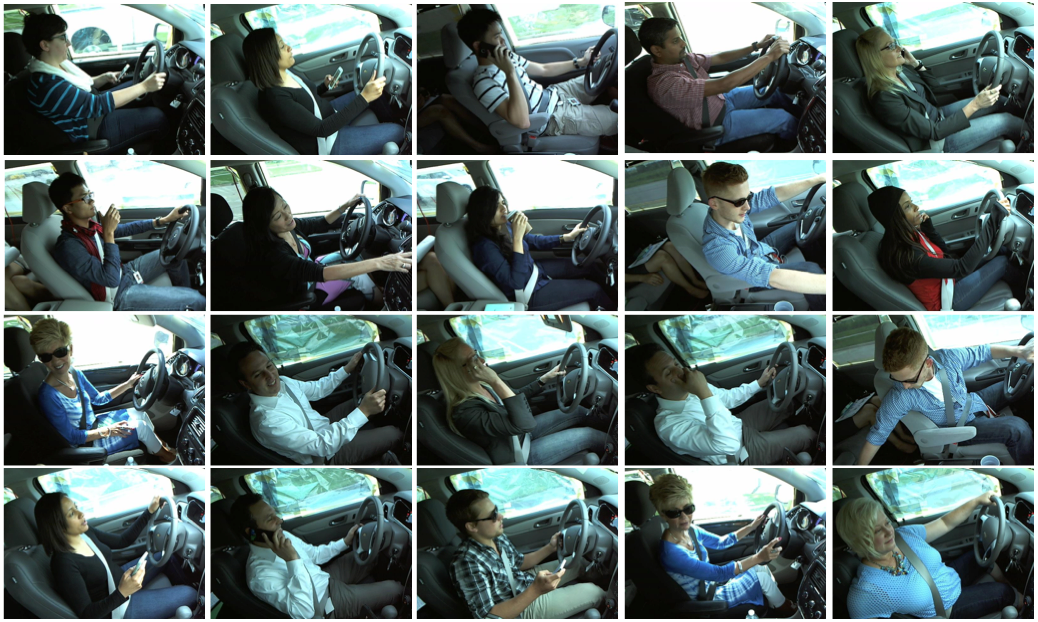
\includegraphics[width=1\textwidth]{Figures/Chapter4_imagenStateFarm.png}	
  \caption{Ejemplo de fotografías de la base de datos (State Farm).}
\end{figure}

\subsection{Proyección sobre un espacio de dimensión 20}

\underline{\textbf{1) Cotas para $\rho^*$}}

En el capítulo 2 se presentaron cotas para $\rho^*$ y en esta sección se ejemplificará la segunda de ellas para esta base de datos. Se calcularon los eigenvalores de la matriz intraclase (B) y de la matriz entre clases (A). Los 20 eigenvalores más grandes y más pequeños de la primera son \footnote{los eigenvalores menores a $1e^{-10}$ se consideraron numéricamente como 0}:

\begin{center}
\begin{tabular}{ | c | c|  c |c | c|  c |c | c|  c |c | c | c|  c |c | c|  c |c | c|  c |c |} 
\hline
291279 & 172080 & 135390 & 101406 & 42280 & 37705 & 30164 \\
26542 & 24004 & 20359 & 17953 & 16532 & 15259 & 14248 \\
13056 & 12014 & 11291 & 10387 & 10143 & 9486 & \\
\hline
\hline
\end{tabular}
\end{center}

\begin{center}
\begin{tabular}{ | c | c|  c |c | c|  c |c | c|  c |c | c | c|  c |c | c|  c |c | c|  c |c |} 
\hline
116 & 115 & 115 & 114 & 113 & 113 & 112 & 112 & 111 & 111 \\
110 & 109 & 108 & 103 & 101 & 100 & 96 & 93 & 92 & 86 \\
\hline
\hline
\end{tabular}
\end{center}

Mientras que los 9 eigenvalores más grandes de la matriz entre clases (A) son (los demás son 0):

\begin{center}
\begin{tabular}{ | c | c|  c |c | c|  c |c | c|  c |} 
\hline
1085 & 7484 & 4378 & 2794 & 2367 & 1830 & 1544 & 1029 & 748 \\
\hline
\hline
\end{tabular}
\end{center}

Sustituyendo estos valores en la fórmula de las cotas de la raíz, se tiene que:

\begin{equation*}
\frac{\sum_{i = 1}^{p}\lambda_{A_i}}{\sum_{i = 1}^{p}\lambda_{B_i}} \leq \rho^* \leq \frac{\sum_{i = 1}^{p}\lambda_{(A)_i}}{\sum_{i = 1}^{p}\lambda_{(B)_{n-i+1}}}	
\end{equation*}

\begin{equation*}
\frac{33027.3}{1011588} \leq \rho^* \leq \frac{33027.3}{2128.5}
\end{equation*}

\begin{equation*}
0.03265 \leq \rho^* \leq 13.51676
\end{equation*}

De esta manera, se sabe que la solución óptima se encuentra en el intervalo $[0.03265, 13.51676]$. 

\pagebreak
\underline{\textbf{2) Valores de $(\rho^*, f(\rho))$}}

Para el punto inicial de este experimento se utilizará el punto medio del intervalo. Los criterios de paro se fijaron con una tolerancia de $1e^{-10}$ y que las iteraciones sean menor a 50. Con este ejemplo, se obtienen los siguientes resultados para $\rho$ y $f(\rho)$:

\begin{center}
\begin{tabular}{ | c | c|  c |} 
\hline
$iter$ & $\rho$ & $f(\rho)$  \\ 
\hline
\hline
1 & $7.774706$ & $-14,702.39$  \\ 
\hline
2 & $1.263660$ & $4,833.57$  \\ 
\hline
3 & $1.974322$ & $993.75$  \\ 
\hline
4 & $2.201148$ & $48.01451$  \\ 
\hline
5 & $2.213198$ & $0.11282$  \\ 
\hline
6 & $2.213226$ & $6.230598e^{-7}$  \\ 
\hline
7 & $2.213226$ & $-2.097522e^{-11}$  \\ 
\hline
\hline

\end{tabular}
\end{center}

\begin{figure}[!ht]
  \centering
	\includegraphics[width=.75\textwidth]{Figures/Chapter4_Iteraciones_StateFarm.png}	
  \caption{Valores de $\rho$ y $f(\rho)$ para distintas iteraciones (State Farm).}
\end{figure}

\pagebreak
\underline{\textbf{3) Primeras 4 componentes de los datos proyectados}}

Se maximizó la traza del cociente para un espacio de 20 dimensiones. En la figura 3.4 se muestra como se agrupan los individuos del conjunto de entrenamiento conforme las iteraciones avanzan. 
  
\begin{figure}[!ht]
  \centering
	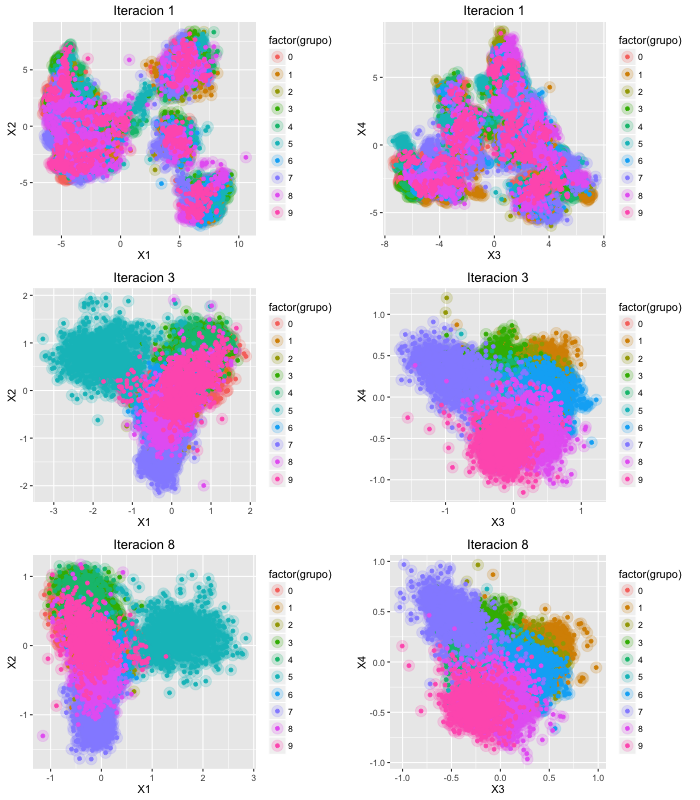
\includegraphics[width=1\textwidth]{Figures/Chapter4_ejemplo20componentes_StateFarm.png}	
  \caption[Ejemplo de proyección en 20 dimensiones (State Farm)]
  {Las dos imágenes superiores son los datos de entrenamiento proyectadas sobre las 4 primeras componentes tras la primer iteración. Las dos intermedias son en la iteración 3 y las últimas 2 son la última iteración.}
\end{figure}

\pagebreak

\subsection{Comparación con otros métodos}

Para la comparación del ADLF implementado con la RLM y el ADL se tomaron las siguientes consideraciones:

\begin{itemize}
\item Las dimensiones a considerar (k) son: 20, 25, 30, 35, 40, 45, 50, 55, 60, 65, 70, 75, 80 y 85
\item El número de variables que entran en cada modelo es el mismo (dada la dimensión $k$)
\item Los modelos se ajustan con el conjunto de entrenamiento y se reporta el error de prueba
\item Se toman las primeras $k$ componentes principales y se aplica el método de manera que sobre esta dimensión, se maximice el cociente de trazas. Después se usó 3-vecinos más cercanos para clasificarlos
\item Para el caso de regresión logística multinomial se elige la clase que tenga una mayor probabilidad posterior de selección. Este modelo solo toma como entrada las primeras $k$ componentes principales
\end{itemize}

\underline{\textbf{1) Tasa de reconocimiento}}

La tasa de reconocimiento se mide como el número de individuos clasificados correctamente entre el número total de individuos del conjunto de test. Como el objetivo de esta sección es observar como se modifica esta tasa con respecto aumenta $k$, se fijó el número de vecinos más cercanos a 3 para el caso de ADL y del ADLF y la dimensionalidad del conjunto de entrenamiento se define como $k$. 

En la figura 3.5 se muestra que el método del ADLF se desempeña mucho mejor que los otros dos. Hay que recordar que este agrupa las clases por lo que es sensato que k-vecinos más cercanos se desempeñe bien con este preprocesamiento. 

\begin{figure}[!ht]
  \centering
	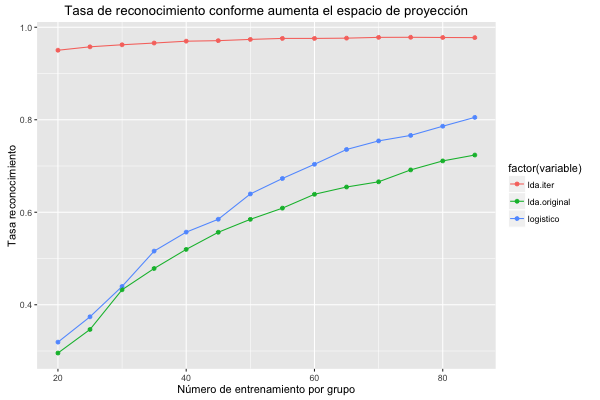
\includegraphics[width=1\textwidth]{Figures/Chapter4_comp_StateFarm.png}	
  \caption[Tasa de reconocimiento de los 3 métodos (State Farm)]
  {En azul se representa el RLM, en verde el ADL y en rojo el método de Newton-Lanczos. En el eje $y$ se muestra la tasa de reconocimiento y en el eje $x$ la dimensión a considerar (k).}
\end{figure}

\pagebreak

\underline{\textbf{2) Tiempo de ejecución}}

A continuación, se comparan los tiempos de ejecución de cada método. Para compararlos justamente, se tomaron 3 distintos:

\begin{itemize}
\item 1) (PCA) Tiempo para calcular los componentes principales del conjunto de entrenamiento
\item 2) (Proyectar) Tiempo para calcular la proyección del conjunto de test
\item 3) (Modelo) Tiempo necesario para hacer las operaciones de cada método

\end{itemize}

\begin{center}
\begin{tabular}{ | c | c |} 
\hline
 PCA (en seg) & Proyectar (en seg)\\ 
\hline
\hline
$178.602$ & $3.112$ \\ 
\hline
\hline
\end{tabular}
\end{center}

\begin{center}
\begin{tabular}{ | c | c | c | c | c | c | c | c |} 
\hline
Comp & lda.iter & logístico & lda.orig   & Comp & lda.iter & logístico & lda.orig   \\ 
\hline
\hline
$20$ & $0.0372$ & $3.1100$ & $0.0696$ & $55$ & $0.1050$ & $9.6192$ & $0.2304$ \\
$25$ & $0.0454$ & $3.6184$ & $0.0984$ & $60$ & $0.1114$ & $10.5422$ & $0.2904$ \\
$30$ & $0.0566$ & $6.3038$ & $0.1054$ & $65$ & $0.1358$ & $11.7946$ & $0.3200$ \\
$35$ & $0.0630$ & $6.9988$ & $0.1386$ & $70$ & $0.1378$ & $12.5136$ & $0.3400$ \\
$40$ & $0.0744$ & $7.7222$ & $0.1764$ & $75$ & $0.1422$ & $13.1488$ & $0.3788$ \\
$45$ & $0.1038$ & $8.6158$ & $0.2116$ & $80$ & $0.1522$ & $14.0320$ & $0.4220$ \\
$50$ & $0.0954$ & $9.1860$ & $0.1996$ & $85$ & $0.1644$ & $13.9156$ & $0.4920$ \\
\hline
\hline
\end{tabular}
\end{center}

El tiempo está en segundos (s).

\begin{figure}[!ht]
  \centering
  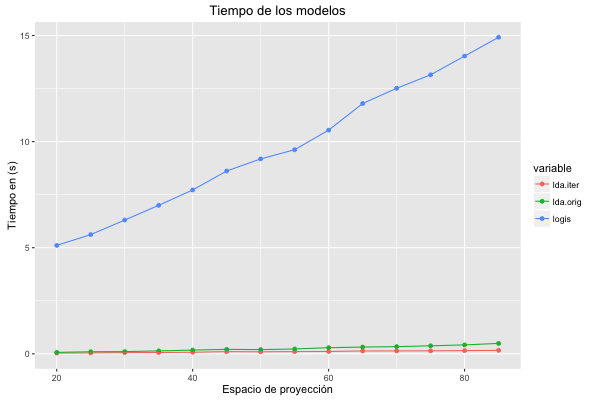
\includegraphics[width=.95\textwidth]{Figures/Chapter4_profilingStateFarm.png} 
  \caption[Tiempo de cómputo (State Farm)]
  {Tiempo requerido para cada método. En el eje $x$ se encuentra el número de componentes tomadas, en el $y$ el tiempo en segundos}
\end{figure}

Para cada iteración del método de Newton-Lanczos, se calcularon todos los eigenvalores ya que al no calcularlos, solo se tendrá una aproximación a sus valores y sus eigenvectores. Por este motivo, se decidió sacrificar tiempo de cómputo por precisión.

\section{Base de datos Otto Group}


Ahora se analizará la base de artículos de \textit{Otto Group}, una compañía de comercio electrónico con presencia en más de 20 países. Actualmente la compañía tiene problemas con el clasificador que utilizan, ya que artículos muy parecidos están asignados en grupos distintos, por lo que desean reducir el error de clasificación. La base consta de 61,878 productos que pertenecen a 9 clases distintas, entre ellas moda, electrónicos, etc. De este número se seleccionaron a 19,000 (1,900 de cada clase) para el análisis. Cada artículo tiene asociado 93 columnas con características numéricas, de las cuales no se proporcionó descripción. La base fue liberada en la plataforma de \textit{Kaggle} con el objetivo de encontrar un clasificador para los artículos de su base de datos. Puede descargarse de la página Web \textit{https://www.kaggle.com/c/otto-group-product-classification-challenge}, cuyo link sigue vigente al 30 de julio del 2016.

La base de datos está en un formato \textit{.csv}, por lo que se requirió la función \textit{read.csv} del paquete $utils$ para cargarlas en R. 

\begin{figure}[!ht]
  \centering
  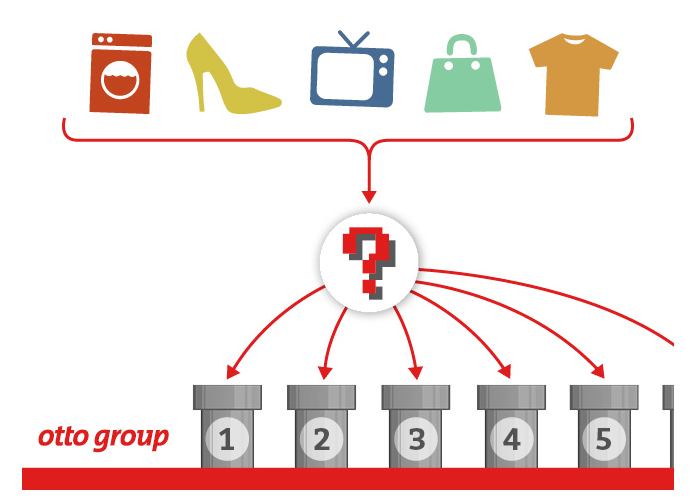
\includegraphics[width=.9\textwidth]{Figures/Chapter4_imagenOtto.png} 
  \caption[Ejemplo de la base de datos (Otto Group)]
  {Base de datos Otto Grup. Su objetivo es clasificar artículos dentro de 9 categorías distintas.}
\end{figure}



\pagebreak

\subsection{Proyección sobre un espacio de dimensión 20}

\underline{\textbf{1) Cotas para $\rho^*$}}

Al igual que el ejemplo de \textit{State Farm}, se ejemplificará la segunda cota presentada en el capítulo 2. Para esto se calcularon los eigenvalores de la matriz intraclase (B) y de la matriz entre clases (A). Respectivamente los 20 eigenvalores más grandes y más pequeños de la primera son: \footnote{los eigenvalores menores a $1e^{-10}$ se consideraron numéricamente como 0}

\begin{center}
\begin{tabular}{ | c | c|  c |c | c|  c |c | c|  c |c | c | c|  c |c | c|  c |c | c|  c |c |} 
\hline
459463 & 284378 & 266461 & 227267 & 203680 & 154707 & 132582 \\
126935 & 121803 & 109100 & 101550 & 93143 & 83423 & 80121 \\
76779 & 74474 & 73521 & 66576 & 64987 & 63187 &\\
\hline
\hline
\end{tabular}
\end{center}

\begin{center}
\begin{tabular}{ | c | c|  c |c | c|  c |c | c|  c |c | c | c|  c |c | c|  c |c | c|  c |c |} 
\hline
195057 & 145551 & 99689 & 86433 & 61103 & 17601 & 8990 & 2517 & 0 & 0 \\
0 & 0 & 0 & 0 & 0 & 0 & 0 & 0 & 0 & 0 \\
\hline
\hline
\end{tabular}
\end{center}

De la misma manera, se calculan los 9 eigenvalores más grandes de la matriz entre clases (Los demás son 0):

\begin{center}
\begin{tabular}{ | c | c|  c |c | c|  c |c | c|  c |} 
\hline
14051 & 12922 & 7775 & 3247 & 3138 & 2849 & 1918 & 1336 & 1317 \\
\hline
\hline
\end{tabular}
\end{center}

Usando las formulas del capítulo 2, se tienen las siguientes cotas para $\rho^*$:

\begin{equation*}
\frac{\sum_{i = 1}^{p}\lambda_{A_i}}{\sum_{i = 1}^{p}\lambda_{B_i}} \leq \rho^* \leq \frac{\sum_{i = 1}^{p}\lambda_{(A)_i}}{\sum_{i = 1}^{p}\lambda_{(B)_{n-i+1}}}  
\end{equation*}

\begin{equation*}
\frac{616,943}{2,864,149} \leq \rho^* \leq \frac{616,943}{61,150}
\end{equation*}

\begin{equation*}
0.215402 \leq \rho^* \leq 10.08895
\end{equation*}


\pagebreak

\underline{\textbf{2) Valores de $(\rho^*, f(\rho^*))$}}

Los criterios de paro se fijaron igual que el ejemplo pasado (tol: $1e^{-10}$ y menos de 50 iteraciones). Para la base de \textit{Otto Group}, se encontraron los siguientes resultados:

\begin{center}
\begin{tabular}{ | c | c|  c |} 
\hline
$iter$ & $\rho$ & $f(\rho)$  \\ 
\hline
\hline
1 & $3.152175$ & $-313,852$  \\ 
\hline
2 & $0.034971$ & $576,318$  \\ 
\hline
3 & $0.558585$ & $250,639$  \\ 
\hline
4 & $1.204773$ & $71,642$  \\ 
\hline
5 & $1.543072$ & $4,015$  \\ 
\hline
6 & $1.564269$ & $13.14$  \\ 
\hline
7 & $1.564349$ & $2.26 e^{-04}$  \\ 
\hline
8 & $1.564349$ & $3.64 e^{-11}$  \\ 
\hline
\hline
\end{tabular}
\end{center}

\begin{figure}[!ht]
  \centering
  \includegraphics[width=.75 \textwidth]{Figures/Chapter4_Iteraciones_Otto.png} 
  \caption{Valores de $\rho$ y $f(\rho)$ para las iteraciones (Otto Group).}
\end{figure}

\pagebreak

\underline{\textbf{3) Primeras 4 componentes de los datos proyectados}}

De nuevo se maximizó la traza del cociente para un espacio de 20 dimensiones. En la figura 3.8 se muestra como se agrupan los individuos del conjunto de entrenamiento conforme las iteraciones aumentan.

\begin{figure}[!ht]
  \centering
  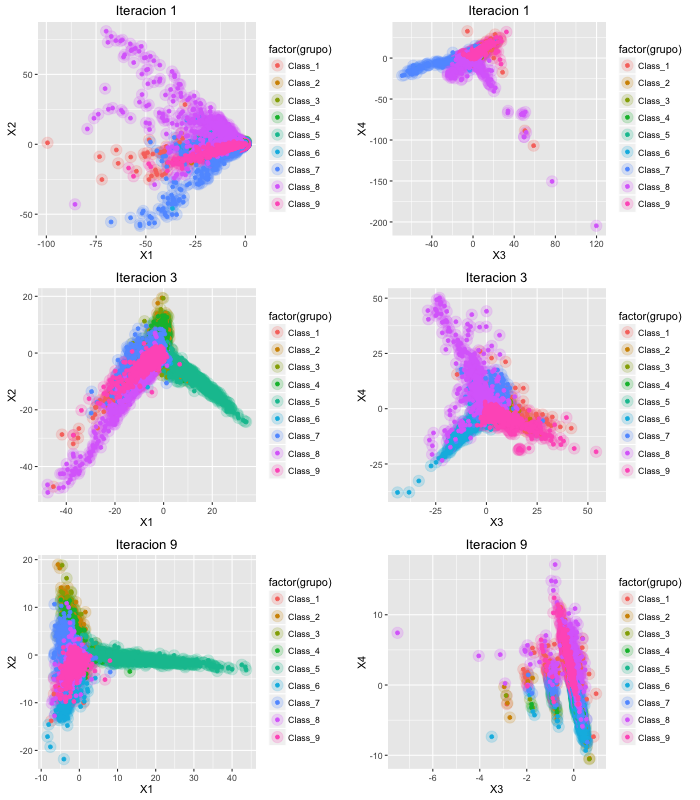
\includegraphics[width=1\textwidth]{Figures/Chapter4_ejemplo20componentes_Otto.png} 
  \caption[Ejemplo de proyección en 20 dimensiones (Otto Group)]
  {Las dos imágenes superiores son los datos de entrenamiento proyectadas sobre las 4 primeras componentes tras la primer iteración. Las dos intermedias son en la iteración 3 y las últimas 2 son la última iteración.}
\end{figure}


\subsection{Comparación con otros métodos}

De la misma forma que el ejemplo pasado se compararon los métodos en este caso. Las dimensiones a considerar k = 20, 25, 30, 35, 40, 45, 50, 55, 60, 65, 70, 75, 80 y 85. 

\underline{\textbf{1) Tasa de reconocimiento}}

\begin{figure}[!ht]
  \centering
  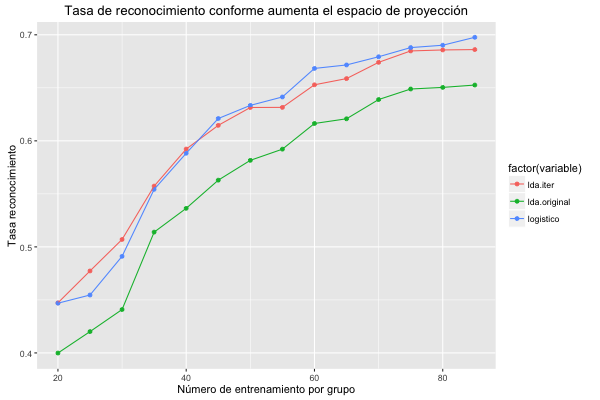
\includegraphics[width=1\textwidth]{Figures/Chapter4_comp_Otto.png} 
  \caption[Tasa de reconocimiento de los 3 métodos (Otto Group)]
  {En azul se representa el RLM, en verde el ADL y en rojo el método de Newton-Lanczos. En el eje $y$ se muestra la tasa de reconocimiento y en el eje $x$ la dimensión a considerar (k).}
\end{figure}

En la figura 3.9 se observa que el método de ADLF compite con el método de RLM y por debajo se encuentra el LDA. Para más de 80 componentes el método de ADLF supera la barrera del 70\% de clasificación. Hay que tomar en cuenta que el número de clases son 9, por lo que una clasificación aleatoria acertaría colamente en el 11.11\%.

\pagebreak
\underline{\textbf{2) Tiempo de ejecución}}
Para el conjunto de datos no se realizó componentes principales; por esto solo se reportan el tiempo que tomó para cada modelo.

\begin{center}
\begin{tabular}{ | c | c | c | c | c | c | c | c |} 
\hline
Comp & lda.iter & logístico & lda.orig   & Comp & lda.iter & logístico & lda.orig   \\ 
\hline
\hline
$20$ & $0.0276$ & $2.7682$ & $0.0534$ & $55$ & $0.0746$ & $6.8098$ & $0.1694$ \\
$25$ & $0.0316$ & $3.5466$ & $0.0690$ & $60$ & $0.0806$ & $7.4876$ & $0.2314$ \\
$30$ & $0.0428$ & $3.9798$ & $0.0830$ & $65$ & $0.1166$ & $8.4616$ & $0.2250$ \\
$35$ & $0.0468$ & $3.8974$ & $0.1102$ & $70$ & $0.1034$ & $9.5988$ & $0.2714$ \\
$40$ & $0.0544$ & $3.7446$ & $0.1134$ & $75$ & $0.1174$ & $9.7264$ & $0.2738$ \\
$45$ & $0.0590$ & $3.4342$ & $0.1308$ & $80$ & $0.1140$ & $10.0674$ & $0.3002$ \\
$50$ & $0.0676$ & $6.0322$ & $0.1492$ & $85$ & $0.1298$ & $10.7434$ & $0.3502$ \\
\hline
\hline
\end{tabular}
\end{center}

El tiempo está en segundos (s).

\begin{figure}[!ht]
  \centering
  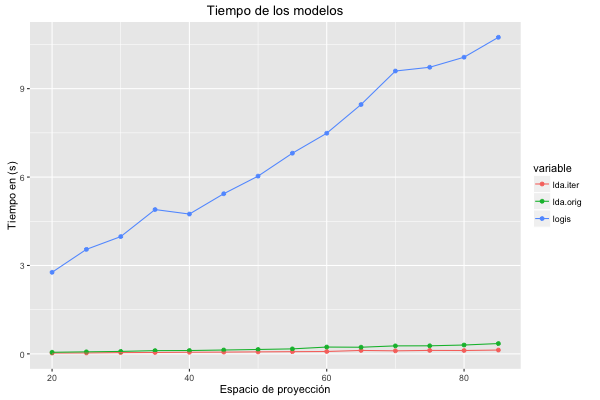
\includegraphics[width=.95\textwidth]{Figures/Chapter4_profilingOtto.png} 
  \caption[Tiempo de cómputo (Otto Group)]
  {Tiempo requerido para cada método. En el eje $x$ se encuentra el número de componentes tomadas, en el $y$ el tiempo en segundos.}
\end{figure}

Para cada iteración del método de Newton-Lanczos, se calcularon todos los eigenvalores ya que al no calcular todos, solo se tendrá una aproximación a sus valores y sus eigenvectores. Por este motivo, se decidió sacrificar tiempo de cómputo por precisión.



